\section{Introduction}

La pyrite, de formule chimique \ce{FeS2}, est plus connue sous le nom de «~pierre à feu~». Elle doit d'ailleurs son nom à sa capacité à produire des étincelles lorsqu'on la frotte ou qu'on la soumet à des chocs avec certains autres matériaux. Longtemps surnommée «~l'or des fous~» de par sa teinte et son aspect qui ont sûrement trompé plus d'un chercheur d'or, la pyrite est aujourd'hui particulièrement utilisée en joaillerie ou dans l'industrie chimique, pour la fabrication d'acide sulfurique. \fxnote{Citation needed}\\
On la trouve naturellement en quantités relativement abondantes dans des gisements à des endroits très divers, en Europe comme en Amérique (lieu d'une «~ruée vers l'or~» au XIXe siècle). Bien qu'elle soit souvent mélangée, par exemple à d'autres composés proches où le fer est substitué par d'autres métaux, il est également possible d'extraire des monocristaux de \ce{FeS2} de taille assez importante sous forme de cubes aux faces lisses ou sous forme de pentagono-dodécaèdres.

\begin{figure}
\caption{Photos d'échantillons cubique et dodécaédrique de cristaux de pyrite.}
\includegraphics{figures/fig1}
\end{figure}

La pyrite fait donc partie des minéraux que l'on connaît et que l'on a utilisé depuis assez longtemps pour ses propriétés macroscopiques, avant-même de comprendre ses propriétés mésoscopiques et \textit{a fortiori} nanoscopiques.
En réalité, ce cristal a été un des premiers objets d'études de la cristallographie moderne au XXème siècle.\\
Dans cet article, on s'attachera à redéterminer par des expériences de diffraction de rayons X, la structure cristallographique complète de la pyrite, en partant d'une étude macroscopique et jusqu'à retrouver son groupe d'espace et ses paramètres de maille.
% But de l'article : déterminer la structure cristallographique complète de la pyrite

\section{Analyse préalable des symétries cristallines}
% Étude préliminaire : Forme des monocristaux
% Éléments de symétrie et groupe ponctuel du cube
% Éléments de symétrie et groupe ponctuel du pentagono-dodécaèdre

Une étude préalable des symétries des cristaux de pyrite (\ce{FeS2}) sous ses deux principaux faciès cubique et pentagono-dodécaédrique peut permettre de guider le reste de l'étude de ce composé et les expériences (et éventuellement de comprendre l'existence de ces deux conformations).\\
Le cube est le système cristallin ayant le plus d'éléments de symétrie. Il possède~:
\begin{itemize}
    \item 3 axes de rotation d'ordre 4, parallèles aux directions \hmn{<001>} et 3 miroirs orthogonaux à ces axes,
    \item 4 axes de roto-inversion\fxnote{Vérifier} d'ordre 3, le long des diagonales \hmn{<111>},
    \item 6 axes de rotation d'ordre 2, parallèles aux diagonales des faces de directions \hmn{<011>} et 6 miroirs orthogonaux à ces axes,
    \item l'élément de centrosymétrie.
\end{itemize}
Cette combinaison d'éléments de symétrie peut s'écrire en notation d'Hermann-Mauguin sous la forme~:
\[
\hmn{*4 -3 *2}
\]
ou sous la forme condensée \hmn{m-3m}.

% \begin{figure*}[!bt]
%   \centering
%   \subfloat[Dummy sub\label{subfig-1:dummy}]{%
%     \rule{4cm}{3cm}
%   }
%   \subfloat[Dummy sub\label{subfig-2:dummy}]{%
%     \rule{4cm}{3cm}
%   }
%   \caption{Dummy figure with subfigures}\label{fig:dummy}
% \end{figure*}
En observant les éléments de symétrie du pentagono-dodécaèdre, on arrive à en retrouver certains en commun avec le cube, dont on se sert comme base pour désigner les directions des axes. La forme spécifique de pentagono-dodécaèdre prise par la pyrite (pyritoèdre) - que l'on sait différente du dodécaèdre régulier pour éviter tout axe de rotation d'ordre 5, incompatible avec la définition classique d'un cristal - comporte donc les symétries suivantes~:
\begin{itemize}
    \item 3 axes de rotation d'ordre 2 selon les directions \hmn{<001>} et 3 miroirs qui leurs sont orthogonaux,
    \item 4 axes de rotation d'ordre 3 selon les directions \hmn{<111>},
    \item l'élément de centrosymétrie.
\end{itemize}
On s'aperçoit alors que l'objet géométrique ainsi obtenu, qui conserve la majeure partie des éléments de symétrie du cube, appartient bien au système cristallin cubique.
La combinaison de ces éléments se note 
\[
\hmn{*2 -3}
\]
ou de manière plus compacte~: \hmn{m-3}.

À l'échelle macroscopique, la pyrite peut prendre les deux formes géométriques présentées ci-dessus. On suppose que cela vient du fait qu'au cours de la croissance, l'assemblage d'objets du système cristallin cubique, même de symétrie légérement inférieure, est favorisé dans les directions permettant de conserver cette symétrie.\\
Autrement dit, le minéral peut croître en gardant simplement ses symétries propres ou en satisfaisant en plus aux contraintes d'une symétrie d'ordre supérieur.\\
Par cette étude macroscopique, on retiendra alors qu'\textit{a priori} le cristal étudié appartient au système cristallin (et réticulaire) cubique et que son groupe ponctuel est celui possédant les éléments de symétrie du pentagono-dodécaèdre, c'est-à-dire \hmn{m-3}.

\section{Méthodes expérimentales}
% Méthodes expérimentales DRX (Laue + SOLEIL/CRISTAL)

Une première expérience de diffraction de rayons X a été réalisée sur des dispositifs spécifiques présents au laboratoire IMPMC de Sorbonne Université, en utilisant la méthode de Laue en transmission (longueur d'onde polychromatique dans un certain intervalle, échantillon fixe pendant la mesure).

La source de rayons X utilisée était un tube à anticathode en cuivre dont la raie \(K_{\alpha_1,\ce{Cu}}\) est de longueur d'onde \(\lambda_{K_{\alpha_1,\ce{Cu}}}=\SI{0.1545}{\nano\metre}\). La cathode en tungstène était excitée avec une tension de \SI{40}{\kilo\volt} (ce qui donne une longueur d'onde minimale \(\lambda_{min} \approx \SI{0.031}{\nano\metre}\)) et un courant de \SI{30}{\milli\ampere}. La lecture du cliché de diffraction de Laue a été réalisée à partir de films réutilisables photosensibles aux RX et numérisés après exposition avec un scanner du même constructeur.\fxnote{Trouver constructeur}

L'échantillon \textit{a priori} monocristallin, placé (après la source) à une distance de \(D = \SI{39}{\milli\metre}\) du détecteur, était monté sur un support permettant un pivot autour de l'axe \hmn{[hkl]}\fxnote{Indiquer direction correcte}.\\
On a positionné visuellement le cristal sous sa forme pyritoédrique de manière à ce que le faisceau incident tape le long d'une arête verticale de direction supposée parallèle à l'axe de pivot. \\
On calcule une erreur angulaire d'orientation \(\varepsilon\) à partir du cliché de Laue obtenu en \figref{fig:laueCliche} par la formule~:
\begin{equation}
\epsilon = \frac{1}{4} \left| \arctan\left( \frac{d_1}{D} \right) - \arctan\left(\frac{d_2}{D}\right) \right|,
\end{equation}
où \(D\) est la distance entre l'échantillon et l'écran, \(d_1\) et \(d_2\) sont les distances entre le centre de l'image et deux tâches de part et d'autre de l'image devant être symétriques l'une par rapport à l'autre.\\
Les résultats de cette méthode sont résumés dans la \tableref{tab:LaueAngleError}.
Le faisceau doit donc arriver le long d'un axe de haute symétrie du cristal, perpendiculairement à la famille de plans \hmn{(hkl)}.\\
\begin{table}
% \caption{Valeurs d'erreur}
\label{tab:LaueAngleError}
\begin{tabular}
  {
    >{$}l<{$}
    S[table-format = 2.3(1)]
  }      % Alignment for each cell: l=left, c=center, r=right
% \midrule
 d_1 / \si{\milli\metre}  & 27,494 \\
 d_2 / \si{\milli\metre}  & 27,438 \\
 D / \si{\degree}         & 0,0137 \\
% \bottomrule
\end{tabular}
\end{table}

Une mesure de diffraction sur synchrotron a également été réalisée sur la ligne CRISTAL du synchrotron SOLEIL.\fxnote{Citer la ligne CRISTAL} La mesure a été effectuée sur un échantillon poudreux de pyrite (\ce{FeS2}) avec un diffractomètre 2 cercles et pour une longueur d'onde incidente monochromatique correspondant à une énergie \(E_i = \SI{17017}{\electronvolt}\), soit \(\lambda_i = \SI{0.07285}{\nano\metre}\).\\
% Le diffractogramme expérimental obtenu sur la \figref{fig:diffractogrammeSOLEIL} est analysé en \secref{sec:}

\section{Analyse des clichés de Laue}
% Observation des éléments de symétrie du cliché de Laue
% Détermination du groupe de Laue -> comparaison avec le groupe ponctuel supposé et limites des clichés de Laue
% => Diffractogramme sur synchrotron (justifications)

On a vu que les cristaux de pyrite \ce{FeS2} adoptaient une forme cubique ou pentagono-dodécaédrique et on en a déduit que le système réticulaire était le système cubique. \\
L'analyse des clichés de Laue doit permettre, à partir de cette hypothèse, de retrouver le groupe ponctuel identifié précédemment.

\begin{figure}
\caption{Cliché de Laue obtenu par DRX sur un cristal de pyrite orienté de telle manière que le faisceau incident soit orthogonal aux plans \hmn{(hkl)}. On repère assez facilement l'axe de rotation d'ordre 2 et deux miroirs orthogonaux entre eux et contenant l'axe.}
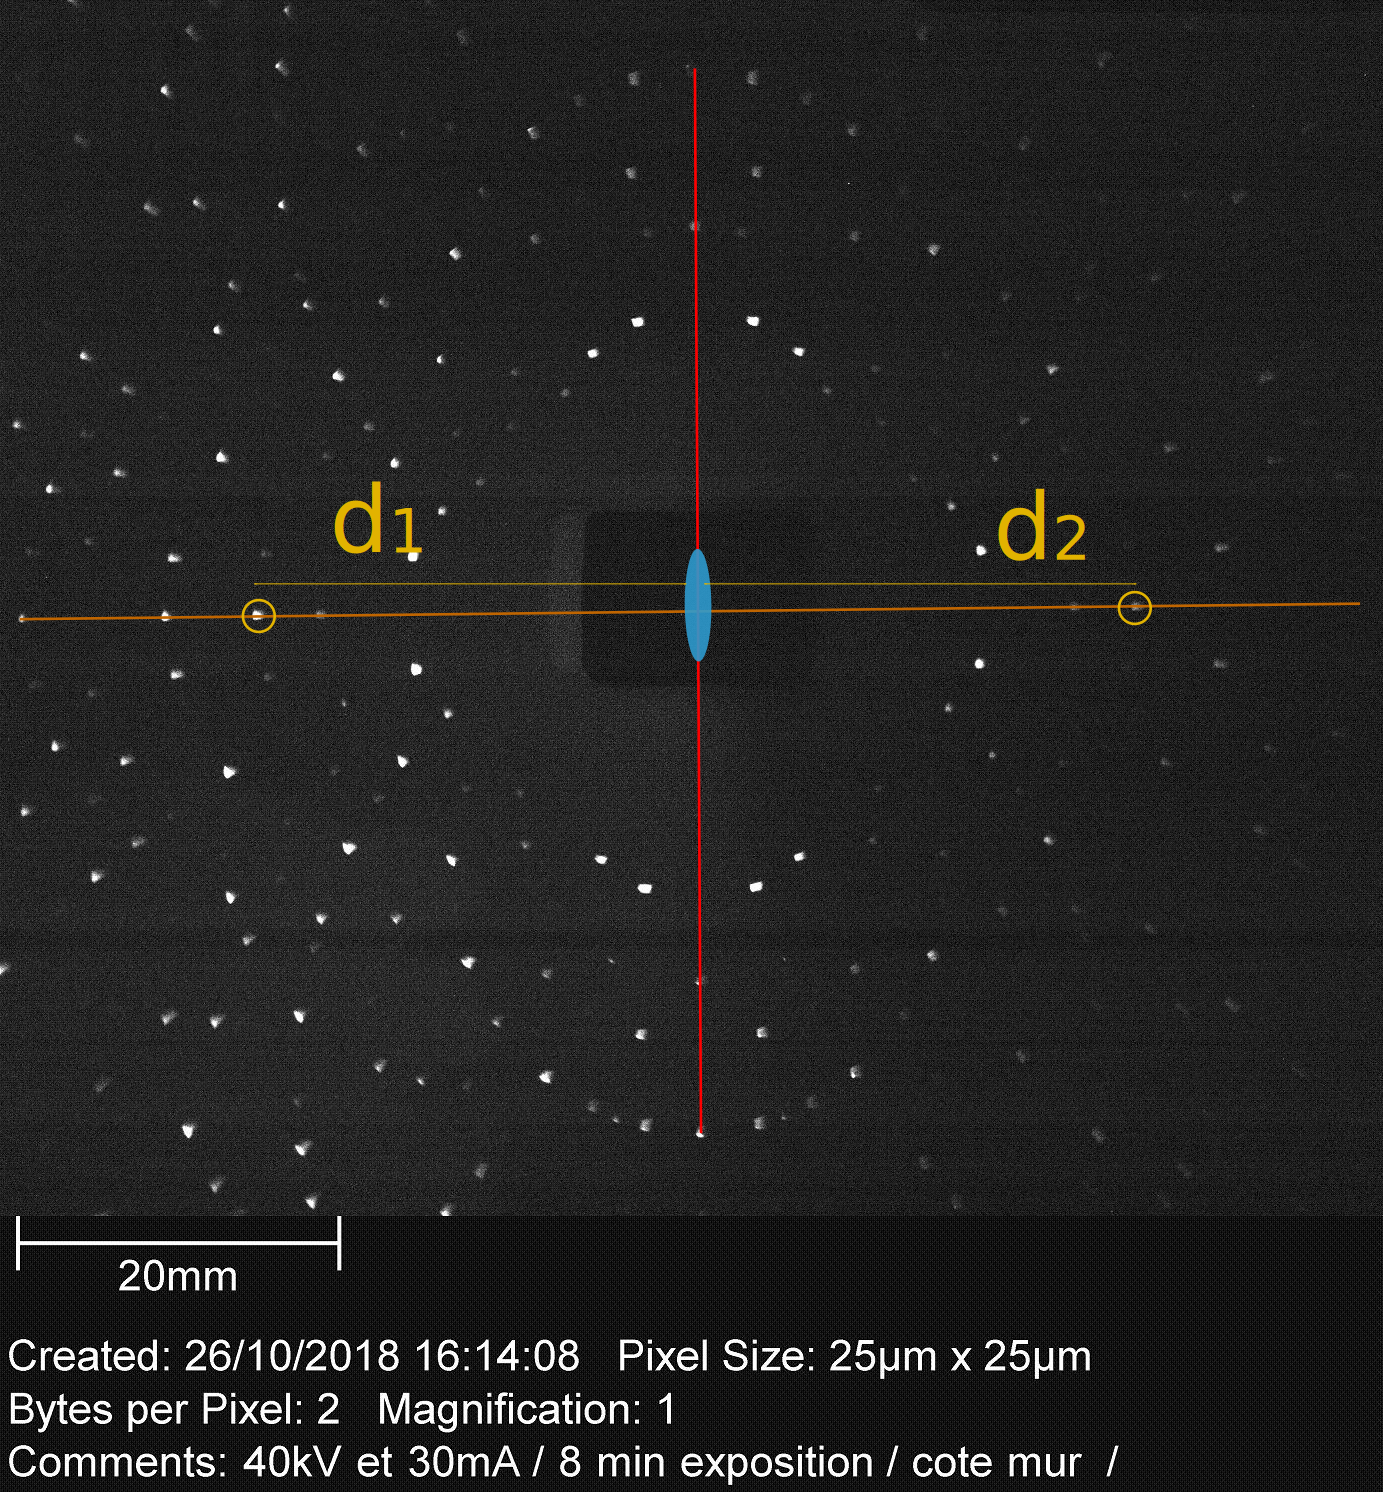
\includegraphics[width=0.85\columnwidth]{figures/Laue_Pyrite_3_symetries}
\label{fig:laueCliche}
\end{figure}

\subsubsection{Symétries, classe de Laue et groupe ponctuel}

Sur la figure de diffraction obtenue en \figref{fig:laueCliche}, on relève un axe de rotation d'ordre 2 et deux miroirs orthogonaux entre eux qui contiennent cet axe.
Il est important de noter qu'il ne s'agit pas d'un axe de rotation d'ordre 4, mais bien d'ordre 2, du fait de la présence/absence de certaines tâches lorsque l'on applique des rotations de \SI{\pi/2}{\radian} (axe d'ordre \hmn{4}) au lieu de \SI{\pi}{\radian} (axe d'ordre \hmn{2}).

La configuration de l'expérience avec le faisceau incident parallèle à un des axes de rotation d'ordre 2 du cristal et deux miroirs orthogonaux, est telle qu'il est normal que l'on ne voit pas d'axes de rotation d'ordre 3 et que l'on retrouve les éléments de symétrie macroscopiques\cite{JJRousseau2007}.\\
Notons que pour retrouver tous les axes de symétrie du cristal et déterminer la classe de Laue sans hypothèse préalable, il aurait fallu faire plusieurs clichés en tournant l'échantillon dans différentes directions.

En regardant les tables de correspondance entre systèmes réticulaires, classes de Laue et groupes ponctuels\cite{IUCrLaueClass,ShmueliIUCr2016}, on voit que le système cubique n'offre que deux classes de Laue possibles~: \hmn{m-3} ou \hmn{m-3m}.
La seconde imposant la présence d'un axe de rotation d'ordre 4 est, de fait, incompatible avec le cliché obtenu.\\
Les clichés de Laue sont nécessairement centrosymétriques d'après la loi de Friedel \fxnote{Citation needed.}, et on ne peut donc pas savoir l'on a affaire à groupe ponctuel centrosymétrique ou non. Dans notre cas, ceci laisse deux groupes ponctuels possibles, associés à la classe de Laue \hmn{m-3}~: \hmn{23} ou \hmn{m-3}.\fxnote{Fix hmn spacing.}

Pour déterminer lequel de ces groupes ponctuels est celui de la pyrite (\ce{FeS2}), on se réfère à nouveau aux symmétries du cristal repérées précédemment.
Puisque ce dernier comporte un centre d'inversion et de manière plus évidente des miroirs, on retrouve bien le groupe ponctuel pré-supposé~: \hmn{m-3}.

\subsection{Pour aller plus loin}

% Erreur d'angle


Pour aller plus loin dans la détermination complète de la structure du cristal, on se propose d'utiliser une autre technique, de diffraction de poudre, sur synchrotron.\\
La diffraction de poudre doit permettre de remonter assez facilement jusqu'au mode de réseau, au groupe d'espace et au paramètre de maille cubique de la pyrite.\\
Par ailleurs, l

\section{Obtention du mode de réseau}
% Tableau des 10 premières raies : numéro des raies (h²+k²+l²), indices (hkl), angles 2*theta, d_hkl, d_i+1/d_i, paramètre de maille
% Lecture des positions angulaires (2*theta) des 10 premières raies
% Calcul des distances inter-réticulaires (Loi de Bragg)
% Calcul des valeurs de rapport entre distances inter-réticulaires (di+1/di)
% Intérêt de ces rapports et comparaison des valeurs expérimentales avec des rapports calculés
% Obtention des indices hkl pour chacune des raies et détermination du mode de réseau (primitif, sinon il y aurait plus d'extinctions -> facteur de structure décomposé en mode+motif)

\section{Calcul du paramètre de maille cubique}
% Détermination du paramètre de maille cubique à partir des d_hkl (formule)
% Moyenne et écart-type de a

\section{Détermination du groupe d'espace}
% Remarque sur le rapport à valeur étrange et explication sur la raie manquante
% Autres directions manquantes sur le diffractogramme
% Parité des directions manquantes et comparaison avec les IToC (annexe 3)
% Déduction du groupe d'espace
% Explication extinctions élément de symétrie (élément translatoire => facteur de structure)

\section{Conclusion}
% Positions atomiques (motif), sites de Wyckoff, ...
% Modèle VESTA
% Comparaison diagramme poudres VESTA vs expérimental SOLEIL
% Conclusion et perspectives

